In this section, we discuss the challenges that we may encounter when we can only access the source model. Then we demonstrate the learning scenarios and proposed solutions in this thesis.

\subsection{Challenges}
Despite for the general challenges in transfer learning, in our HTL settings, there are some new challenges in this thesis.

The first challenge is \textbf{knowledge representation}, i.e. how to obtain the source knowledge when we are not able to access to the source data. When source data is accessible, the source knowledge is relatively explicit and we can easily obtain the source knowledge by either analyzing the source data distribution or make use of the source data to help training the target mode. The knowledge of the source domain is implicit and encoded in the source model using certain learning algorithms. How to effectively extract the source knowledge from the models is challenging.

The second challenge is \textbf{knowledge expressiveness}, i.e. how to leverage the source knowledge to help training the target model. As the source knowledge is implicit, how to effectively leverage the source knowledge and improve the transfer performance is also important. We also expect that the source knowledge extracted from the source model should be as general as possible so that the source knowledge can be extracted from different types of source model. Therefore, the our transfer learning algorithm can work in many situation. 

The last challenge is \textbf{knowledge regularization} i.e. how to guarantee the performance of our transfer method. 
Humans appear to have mechanisms for deciding when to transfer information, selecting appropriate sources of knowledge, and determining the appropriate level of abstraction \cite{torrey2009transfer}. 
A basic criterion for the knowledge transfer process is that leveraging the knowledge from the source model should not hurt the performance of the target model. Negative transfer \cite{pan2010survey} happens when the performance of target model degrades after receiving the knowledge from the source domain and how to avoid negative transfer is still an open question to all transfer learning researchers. The absence of the source data makes the situation more complicated.

\subsection{Two Transfer Learning Scenarios}
In this thesis, we mainly focus on two transfer learning scenarios: inductive transfer learning for new classes and domain adaptation. The definition of the two scenarios is as follows:
\begin{definition}{\textbf{Domain Adaptation}}
	Let $X$ be the input space and $Y$ be output space. Given the source domain $D_s$ and the target learning task $D_t$ with marginal distribution $P(X_s)$ and $P(X_t)$, we assume that $D_s$ and $D_t$ share the same conditional distribution $P(Y|X)$. The goal of Domain Adaptation is to learn the $P(X_t|Y_t)$ for the target task with the help of $D_s$.
\end{definition}

\begin{definition}{\textbf{Inductive Transfer Learning}}\cite{pan2010survey}
	Given a source domain $D_s$ and the source learning task $T_s$, a target domian $D_s$ and the target learning task $D_t$, inductive transfer learning aims to help improve the learning of the target task function $f_t(\cdot)$ in $D_t$ using the knowledge from $D_s$ and $D_s$ where $D_s \neq D_t$.
\end{definition}

The major difference between the two transfer learning scenarios is that in inductive transfer learning, the source and target tasks are two different but related tasks (e.g. from sport car to heavy truck) while in domain adaptation, the source and target tasks are the same task but with different marginal distributions (e.g. from the animation dog to the real dog). 

\begin{figure}[h]
	\centering
	\subfloat[Domain Adaptation]{\includegraphics[scale=.4]{introduction/fig/da.png}}
	\qquad
	\subfloat[Inductive transfer learning the new class]{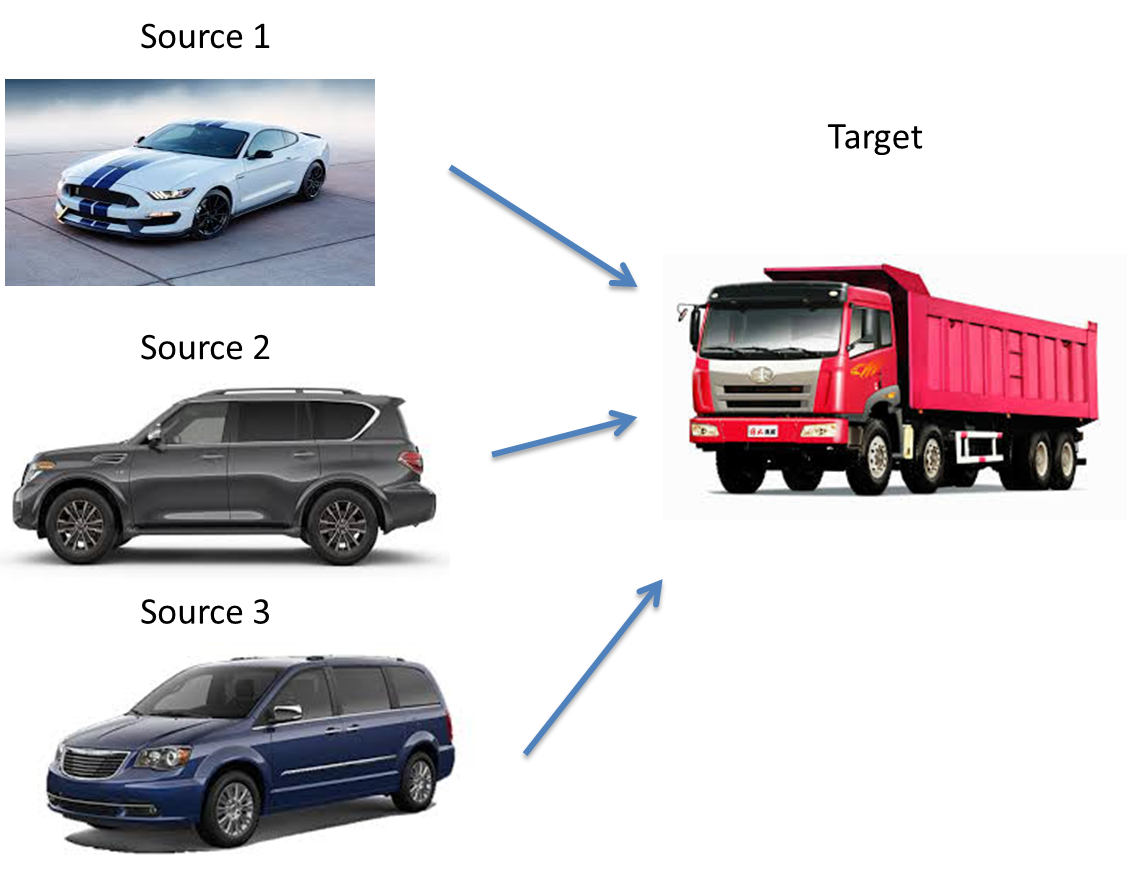
\includegraphics[scale=.33]{introduction/fig/ind.png}}
	\caption{Difference between two transfer learning scenarios}\label{fig:intro:cmp}
\end{figure}


\subsection{Proposed Methods}
There are 3 methods proposed in this thesis, one in inductive transfer learning for new classes and two methods in domain adaptation.


In chapter \ref{sec:pakdd}, we extend the previous methods in HTL which are limited to using SVMs as the source model and propose a novel method \textbf{Effective Multi-class Transfer Learning} (EMTLe) for supervised domain adaptation. We use the output of the source model as the auxiliary bias to adjust the target model. Therefore, EMTLe can leverage the source model from any source classifier that can generate predict class probability.

In chapter \ref{sec:aaai}, we investigate the problem of semi-supervised domain adaptation and propose a novel framework \textbf{Generalized Distillation Semi-supervised Domain Adaptation} (GDSDA) that can effectively transfer the knowledge from the source model under the semi-supervised domain adaptation scenario. 

In chapter \ref{sec:cnn}, we use the deep neural network to solve the transfer learning problem for food recognition. We use GoogLeNet trained from ImageNet of 1000 classes as our source model and two food databases as our target task, containing 101 classes and 265 classes respectively. We use the parameters in the original GoogLeNet as a prior and fine-tune it on our target task to achieve the improved performance.